\begin{figure} [H]
	\begin{center}
		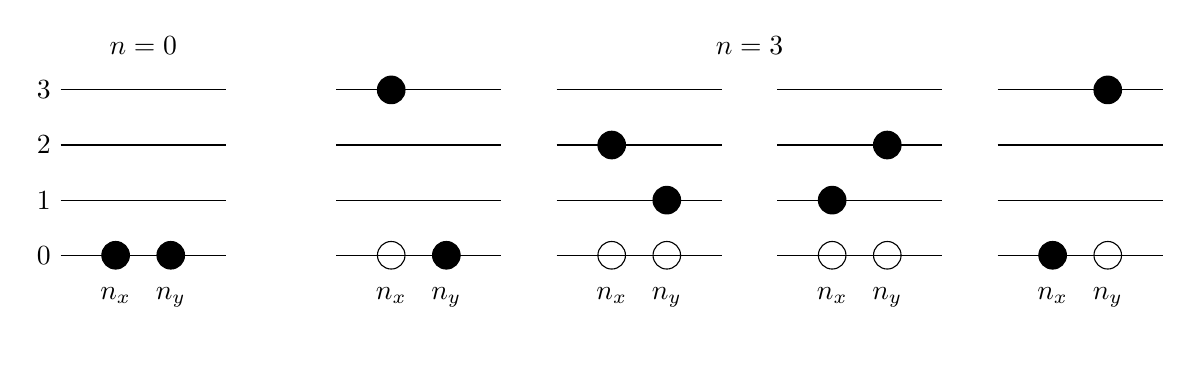
\begin{tikzpicture}[scale=0.7]
		\begin{scope}
		\foreach \i in {0,...,3}
		{
			\draw (-1,\i) node[anchor=east] {$\i$} --(2,\i);
		}
		\filldraw (0,0) node[anchor=north,inner sep=.4cm] {$n_x$} circle (0.25cm); 
		\filldraw (1,0) node[anchor=north,inner sep=.4cm] {$n_y$} circle (0.25cm);
		\node[] at (0.5,3.8) {$n=0$};
		\end{scope}
		\begin{scope}[xshift=5cm]
		\foreach \i in {0,...,3}
		{
			\draw (-1,\i) --(2,\i);
		}
		\draw (0,0) node[anchor=north,inner sep=.4cm] {$n_x$} circle (0.25cm); 
		\filldraw (1,0) node[anchor=north,inner sep=.4cm] {$n_y$} circle (0.25cm);
		\filldraw (0,3) circle (0.25cm);
		\end{scope}
		\begin{scope}[xshift=9cm]
		\foreach \i in {0,...,3}
		{
			\draw (-1,\i) --(2,\i);
		}
		\draw (0,0) node[anchor=north,inner sep=.4cm] {$n_x$} circle (0.25cm); 
		\draw (1,0) node[anchor=north,inner sep=.4cm] {$n_y$} circle (0.25cm);
		\filldraw (0,2) circle (0.25cm); 
		\filldraw (1,1) circle (0.25cm); 
		\node[] at (2.5,3.8) {$n=3$};
		\end{scope}
		\begin{scope}[xshift=13cm]
		\foreach \i in {0,...,3}
		{
			\draw (-1,\i) --(2,\i);
		}
		\draw (0,0) node[anchor=north,inner sep=.4cm] {$n_x$} circle (0.25cm); 
		\draw (1,0) node[anchor=north,inner sep=.4cm] {$n_y$} circle (0.25cm);
		\filldraw (0,1) circle (0.25cm); 
		\filldraw (1,2) circle (0.25cm); 
		\end{scope}
				\begin{scope}[xshift=17cm]
		\foreach \i in {0,...,3}
		{
			\draw (-1,\i) --(2,\i);
		}
		\filldraw (0,0) node[anchor=north,inner sep=.4cm] {$n_x$} circle (0.25cm); 
		\draw (1,0) node[anchor=north,inner sep=.4cm] {$n_y$} circle (0.25cm);
		\filldraw (1,3) circle (0.25cm); 
		\end{scope}
		\end{tikzpicture}
	\end{center}

	\begin{center}
		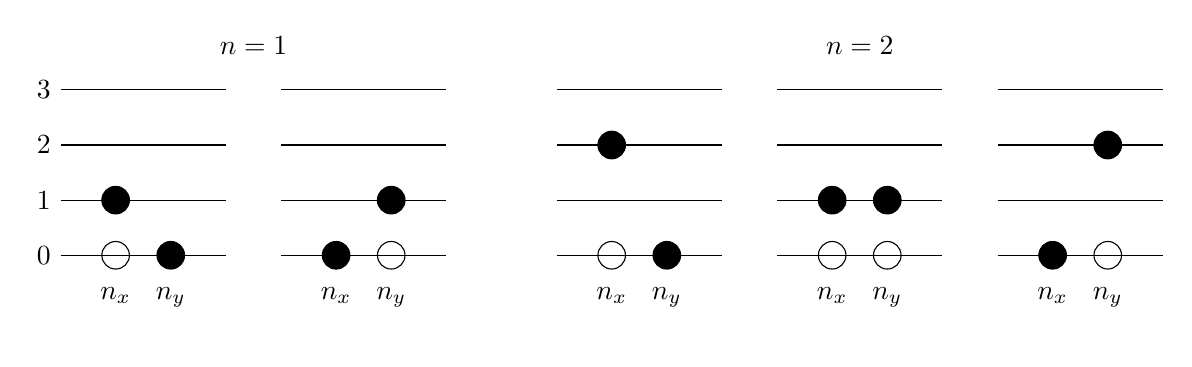
\begin{tikzpicture}[scale=0.7]
		\begin{scope}
		\foreach \i in {0,...,3}
		{
			\draw (-1,\i) node[anchor=east] {$\i$} --(2,\i);
		}
		\draw (0,0) node[anchor=north,inner sep=.4cm] {$n_x$} circle (0.25cm); 
		\filldraw (1,0) node[anchor=north,inner sep=.4cm] {$n_y$} circle (0.25cm);
		\filldraw (0,1) circle (0.25cm);
		\node[] at (2.5,3.8) {$n=1$};
		\end{scope}
		\begin{scope}[xshift=4cm]
		\foreach \i in {1,...,4}
		{
			\draw (-1,\i-1) --(2,\i-1);
		}
		\filldraw (0,0) node[anchor=north,inner sep=.4cm] {$n_x$} circle (0.25cm); 
		\draw (1,0) node[anchor=north,inner sep=.4cm] {$n_y$} circle (0.25cm);
		\filldraw (1,1) circle (0.25cm); 
		\end{scope}
		\begin{scope}[xshift=9cm]
		\foreach \i in {1,...,4}
		{
			\draw (-1,\i-1) --(2,\i-1);
		}
		\draw (0,0) node[anchor=north,inner sep=.4cm] {$n_x$} circle (0.25cm); 
		\filldraw (1,0) node[anchor=north,inner sep=.4cm] {$n_y$} circle (0.25cm);
		\filldraw (0,2) circle (0.25cm);
		\end{scope}
		\begin{scope}[xshift=13cm]
		\foreach \i in {1,...,4}
		{
			\draw (-1,\i-1) --(2,\i-1);
		}
		\draw (0,0) node[anchor=north,inner sep=.4cm] {$n_x$} circle (0.25cm); 
		\draw (1,0) node[anchor=north,inner sep=.4cm] {$n_y$} circle (0.25cm);
		\filldraw (0,1) circle (0.25cm); 
		\filldraw (1,1) circle (0.25cm);
		\node[] at (0.5,3.8) {$n=2$};
		\end{scope}
		\begin{scope}[xshift=17cm]
		\foreach \i in {1,...,4}
		{
			\draw (-1,\i-1) --(2,\i-1);
		}
		\filldraw (0,0) node[anchor=north,inner sep=.4cm] {$n_x$} circle (0.25cm); 
		\draw (1,0) node[anchor=north,inner sep=.4cm] {$n_y$} circle (0.25cm); 
		\filldraw (1,2) circle (0.25cm);
		\end{scope}
		\end{tikzpicture}
	\end{center}
	\caption{Possible states of a two dimensional single quantum dot.}
	\label{fig:schematic_2d}
\end{figure}